% !TEX root = slides.tex

\section{Identification}

\begin{frame}
    \frametitle{Identification}
    \begin{figure}
        \centering
        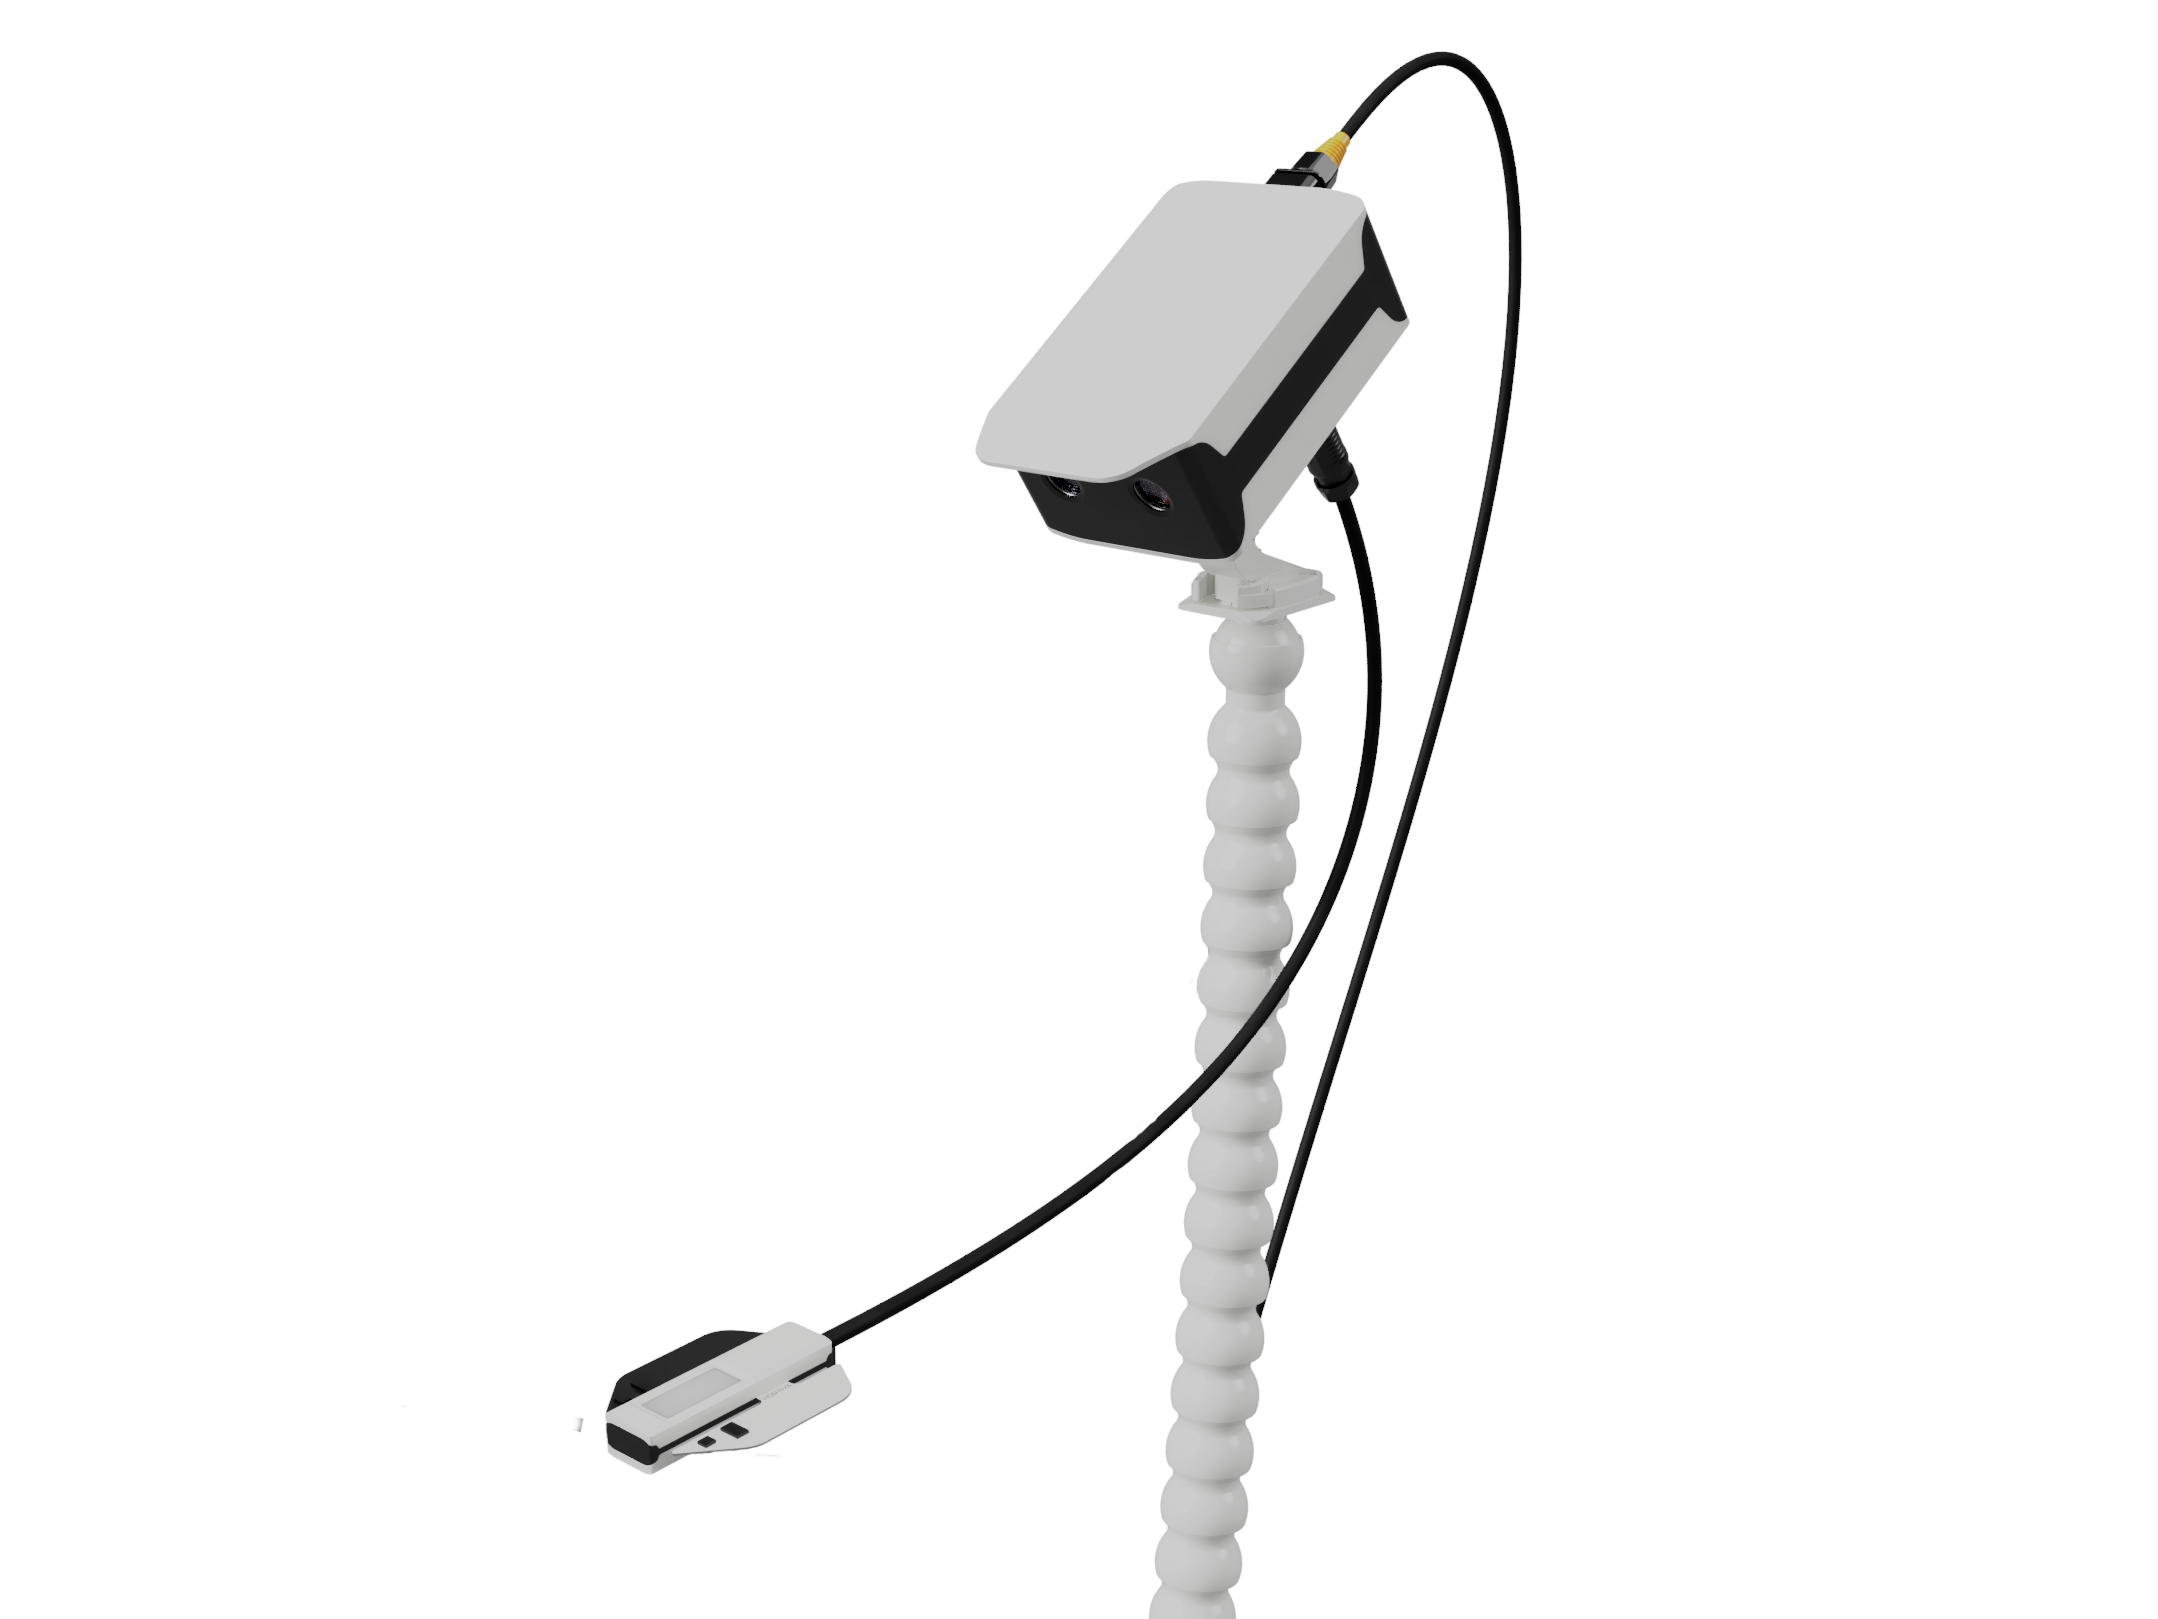
\includegraphics[scale=0.066]{figures/ceres.png}
        \caption{Hortiya sensor system.}
    \end{figure}
\end{frame}

\begin{frame}
    \frametitle{Identification}
    \begin{figure}
        \centering
        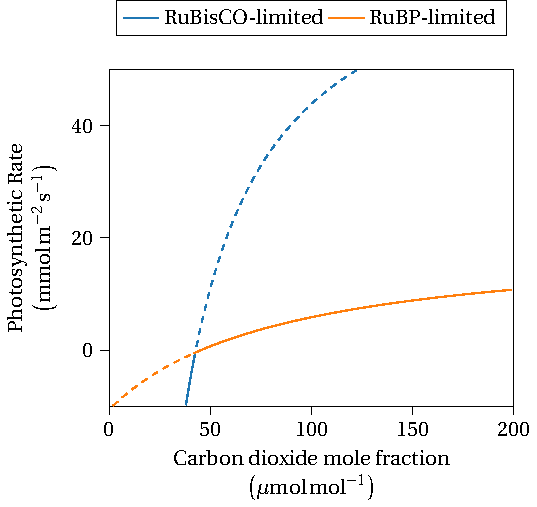
\includegraphics[scale=0.5]{figures/photosynthesis.pdf}
        \caption{RuBisCo- and RuBP-limited photosynthetic rate.}
    \end{figure}
\end{frame}

\begin{frame}
    \frametitle{Identification}
    \begin{figure}
        \centering
        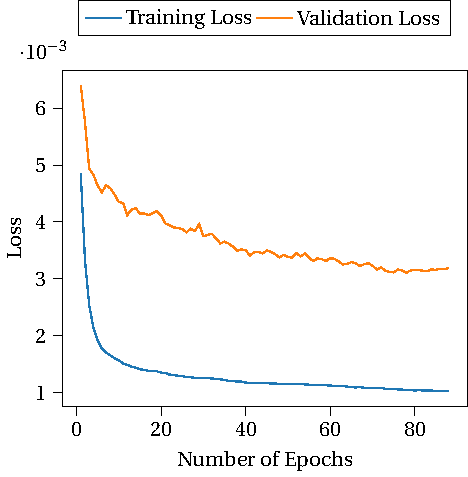
\includegraphics[scale=0.5]{figures/nn2.pdf}
        \caption{Mean losses over the training and validation datasets.}
    \end{figure}
\end{frame}

\begin{frame}
    \frametitle{Identification}
    \begin{figure}
        \centering
        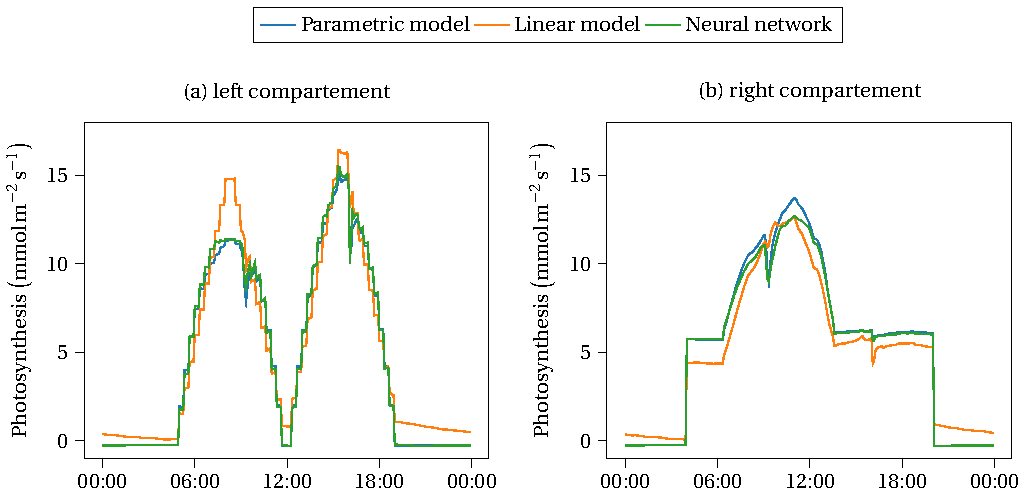
\includegraphics[scale=0.5]{figures/nn3.pdf}
        \caption{Photosynthetic rates for the (a) left and (b) right compartement.}
    \end{figure}
\end{frame}